\chapter{Bilan et Guide d'utilisation du \textit{Clustering Interactif}}
\label{chapter:5-GUIDE}
	
	% Introduction.
	Dans nos études, nous nous sommes intéressés aux assistants conversationnels orientés par tâches et aux méthodes de conception des bases d'apprentissage nécessaires à leur entraînement.
	Dans ce chapitre, nous dressons une synthèse des découvertes et des conseils d'utilisation de notre méthodologie d'annotation basée sur un \texttt{Clustering Interactif} ayant pour but d'assister les experts métiers dans la phase de modélisation des textes en intentions de dialogue.
	
	%%%%%--------------------------------------------------------------------
	%%%%% Section 5.1:
	%%%%%--------------------------------------------------------------------
	\section{Présentation rapide du \textit{Clustering Interactif} et de ses avantages}
		\label{section:5.1-GUIDE-PRESENTATION-RAPIDE}
		
		% Détails de fonctionnement.
		\todo[inline]{
			SECTION À RÉDIGER: \\
			- trouver une base d'apprentissage acceptable, puis corriger manuellement \\
			- intervention d'experts métiers sur la base de leur connaissance métiers \\
			- revues d'annotations basée sur leur connaissance métiers \\
			- aide à la modélisation par le \textit{clustering}
		}
		
		% Constat : expert métier pas à leur place !
		\begin{leftBarReminder}
			% Rappel: Complexité et cycle MATTER
			Nous partons du constat selon lequel la conception d'une base d'apprentissage de textes annotés en intentions est connue pour être complexe, subjective et sensible aux erreurs (voir \textsc{Section~\ref{section:2.3-DEFIS-ANNOTATION}}).
			Pour limiter ces problèmes, le projet de labellisation s'organise autour du cycle \texttt{MATTER} (\cite{pustejovsky-stubbs:2012:natural-language-annotation}) durant lequel une modélisation abstraite des intentions est définie pour d'annoter les données, et cette modélisation peut être affinée ou remise en cause plusieurs fois pour mieux s'adapter le mieux possible aux données du projets (voir \textsc{Section~\ref{section:2.2-ORGANISATION-ANNOTATION}}).
			
			% Besoin d'experts métiers.
			Les experts métiers modélisant et annotant les données ont donc besoin de leur connaissance métier du sujet à traiter, mais aussi de compétences analytiques et techniques pour s'assurer de la qualité de la base d'apprentissage en cours de conception.
			Ainsi, un projet d'annotation devient donc rapidement coûteux, notamment car il demande des formations analytiques à des experts métiers, nécessite l'organisation d'ateliers de modélisation en mode essai-erreur pour trouver une base d'apprentissage stable et pertinente, et fait intervenir des experts métiers sur une abstraction de leurs connaissances du quotidien.
			
			% Remise en cause.
			Au cours de ce doctorat, nous avons questionné cette approche de modélisation, et avons proposé une nouvelle méthodologie d'annotation basée sur un \texttt{Clustering Interactif} dans le but d'impliquer les experts métiers sur leur vrai domaine de connaissances et en leur demandant un minimum de bagages analytiques ou techniques.
		\end{leftBarReminder}
		
		% Proposition de \texttt{Clustering Interactif}.
		Nous proposition de méthodologie d'annotation basée sur un \texttt{Clustering Interactif} repose sur l'alternance de deux étapes clefs : ...
		
		
		\begin{leftBarImportantGreen}
			La \textsc{Figure~\ref{figure:5.1-GUIDE-PRESENTATION-RAPIDE-CLUSTERING-INTERACTIF}} ...
			
			% Figure.
			\begin{figure}[H]
				\centering
				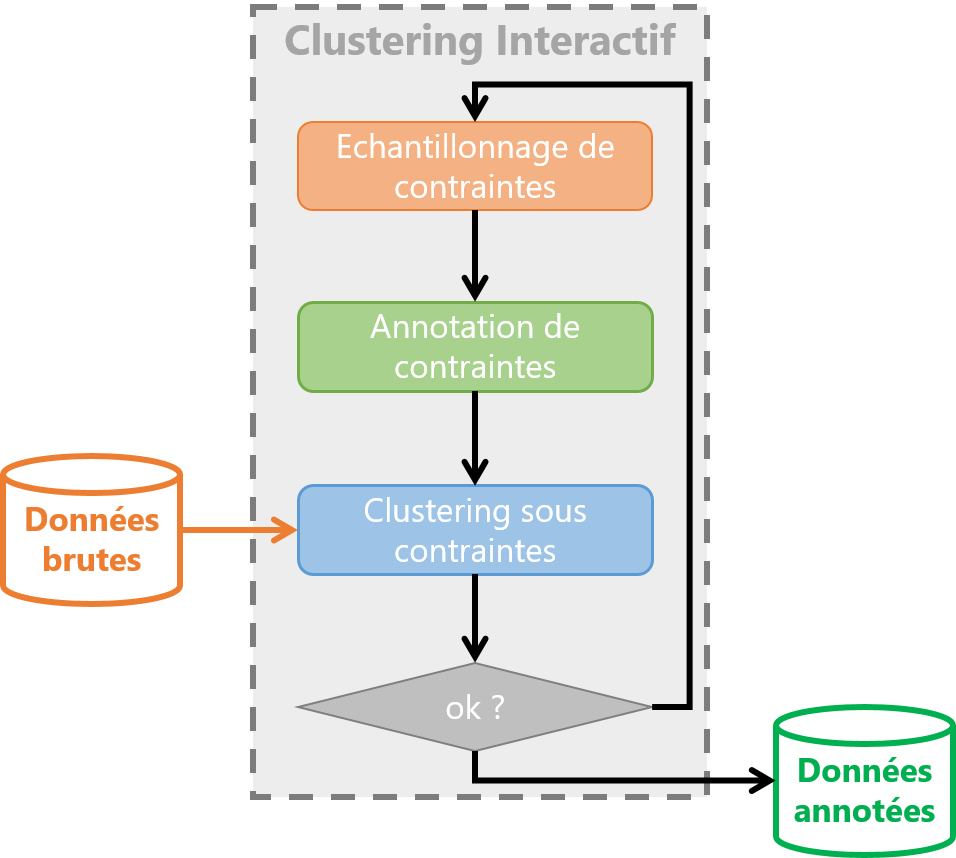
\includegraphics[width=0.95\textwidth]{figures/interactive-clustering-architecture-sequentielle}
				\caption{
					Schéma illustrant l'architecture du \texttt{Clustering Interactif}.
					La boucle principale enchaîne un échantillonnage de couples de données, une annotation de contraintes, et un \textit{clustering} sous contraintes.
				}
				\label{figure:5.1-GUIDE-PRESENTATION-RAPIDE-CLUSTERING-INTERACTIF}
			\end{figure}
		\end{leftBarImportantGreen}
	
	
	%%%%%--------------------------------------------------------------------
	%%%%% Section 5.2:
	%%%%%--------------------------------------------------------------------
	\section{Conseils pour organiser l'annotation}
		\label{section:5.2-GUIDE-ANALYSE}
		\todo[inline]{
			SECTION À RÉDIGER: \\
			- bien définir l'objectif à modéliser (par action ? par objet ?) \\
			- laisser à la mach \\
			- faire référence aux maximes de \cite{leech:1993:corpus-annotation-schemes} ?
			1. VOIR LA DONNEE NON PRETRAITEE: It should always be possible to come back to initial data (example BC). Note: can be hard after normalization ("l'arbre !" vs "le arbre", etc.) \\
			2. ANNOTER DES DIFFERENCES VISIBLES: Annotations should be extractable from the text \\
			3. DOCUMENTER L'AJOUT DE CONTRAINTES: The annotation procedure should be documented (ex: Brown Corpus annotation guide, Penn Tree Bank annotation guide) \\
			4. DOCUMENTER LES COMPETENCES DES ANNOTATEURS: Mention should be made of the annotator(s) and the way annotation was made (manual/automatic annotation, number of annotators, manually corrected/uncorrected...) \\
			5. SUBJECTIVITE => 3 ANNOTATEURS: Annotation is an act of interpretation (cannot be infallible) \\
			6. MIEUX VAUT NE PAS LIER QUE LIER DE MANIERE AMBIGUE: Annotation schemas should be as independent as possible on formalisms \\
			7. PLUSIEURS VISIONS POSSIBLES, IL FAUT EN CHOISIR UNE ET S'Y TENIR: No annotation schema should consider itself a standard (it possibly becomes one)
		}
	
	
	%%%%%--------------------------------------------------------------------
	%%%%% Section 5.3:
	%%%%%--------------------------------------------------------------------
	\section{Conseils pour analyser les résultats}
		\label{section:5.3-GUIDE-ANALYSE}
		\todo[inline]{
			SECTION À RÉDIGER: \\
			- Cas d'arrêt quand le \textit{clustering} stagne à 5\% : si change pas, alors l'annotation n'a plus d'effet... \\
			- utiliser le graphe de contraintes pour voir les données liées entres elles et les données isolées \\
			- Analyse avec résumer par LLM pour identifier facilement les thématiques qui se dégagent \\
			- Analyse avec FMC pour identifier le vocabulaire qui caractérise chaque thématique \\
			- utiliser ces analyses pour régler le nombres d clusters ?
		}
	
	
	%%%%%--------------------------------------------------------------------
	%%%%% Section 5.4:
	%%%%%--------------------------------------------------------------------
	\section{Conseils pour paramétrer la méthode}
		\label{section:5.4-GUIDE-PARAMETRAGES-ET-COUTS}
		
		
		%%% Paramétrage optimal.
		\paragraph{Paramétrage optimal :}
		
		Grâce au \textsc{Chapitre~\ref{chapter:4-ETUDES}}, nous avons pu mettre en avant un \textbf{paramétrage favori} de notre méthode.
		Il est composé des algorithmes suivants :
		
		\setcounter{localCounterOfFootnoteValue}{\value{footnote}}
		\begin{leftBarImportantGreen}
			\paragraph{Paramétrage favori du \texttt{Clustering Interactif} :}
			\begin{itemize}
				\item \texttt{prep.simple}, c'est-à-dire des \textbf{prétraitements} \textbf{simples} supprimant les minuscules, les ponctuations, les accents et les espaces blancs ;
				\item \texttt{vect.tfidf}, c'est-à-dire une \textbf{vectorisation} basée sur une représentation statistique du vocabulaire à l'aide d'un \textbf{TF-IDF} (\cite{ramos:2003:using-tfidf-determine}) ;
				\item \texttt{clust.kmeans.cop}, c'est-à-dire un \textbf{\textit{clustering} sous contraintes} basé sur l'algorithme \texttt{KMeans} adapté en mode \textbf{\texttt{COP-KMeans}} (\cite{wagstaff-etal:2001:constrained-kmeans-clustering}) ;
				\item \texttt{samp.closest.diff}, c'est-à-dire l'\textbf{échantillonnage de contraintes} concernant des données issues de \textbf{clusters différents} et étant \textbf{les plus proches} les unes des autres.
			\end{itemize}
			Ces implémentations, disponibles dans la librairie \texttt{cognitivefactory-interactive-clustering} \footnotemark, sont détaillées en \textsc{Annexe~\ref{annex:C-ANNEXE-IMPLEMENTATIONS}}.
		\end{leftBarImportantGreen}
		% Rattraper les footnote.
			\stepcounter{localCounterOfFootnoteValue}
			\footnotetext[\value{localCounterOfFootnoteValue}]{
				\url{https://pypi.org/project/cognitivefactory-interactive-clustering/}
			}
			
		Ce paramétrage favori a été choisi sur la base d'un compromis entre un maximum d'efficience (\textsc{Section~\ref{section:4.2-HYPOTHESE-EFFICIENCE}}) et un minimum de coûts (\textsc{Section~\ref{section:4.3-HYPOTHESE-COUTS}})
			
		Un tel paramétrage nécessite un temps de calcul de :
		\begin{equation}
			\label{equation:5.4-GUIDE-PARAMETRAGES-ET-COUTS-TEMPS-CALCUL}
			\texttt{computation\_time}~[s]~\propto~0.17 \cdot \texttt{dataset\_size}
		\end{equation}
			
		
		
		%%% Coûts 
		\begin{equation}
			\label{equation:5.4-GUIDE-PARAMETRAGES-ET-COUTS-TEMPS-UNE-ITERATION-PARALLELE}
			\begin{cases}
				% Computation time.
				\texttt{computation\_time}~[s]&
					~\propto~0.17 \cdot \texttt{dataset\_size}\\
				% Annotation time.
				\texttt{annotation\_time}~[s]&
					~\propto~7.8 \cdot \texttt{batch\_size} \\
				% Batch size.
				\texttt{optimal\_batch\_size}~[\#]&
					~\propto~0.0218 \cdot \texttt{dataset\_size} \\
				% Iterations number.
				\texttt{iterations\_needed}~[\#] &
					~\propto~144.5 \\
				% Total time (parallel).
				\texttt{total\_time(parallel)}~[s] &
						~\propto~24.6 \cdot \texttt{dataset\_size}
			\end{cases}
		\end{equation}
		
		%%% Batch size minimal.
		
		
		%%% Architecture parallèle.
		\begin{leftBarImportantGreen}
			La \textsc{Figure~\ref{figure:5.4-GUIDE-PARAMETRAGES-ET-COUTS-ARCHITECTURE-PARALLELE}} ...
			
			% Figure.
			\begin{figure}[H]
				\centering
				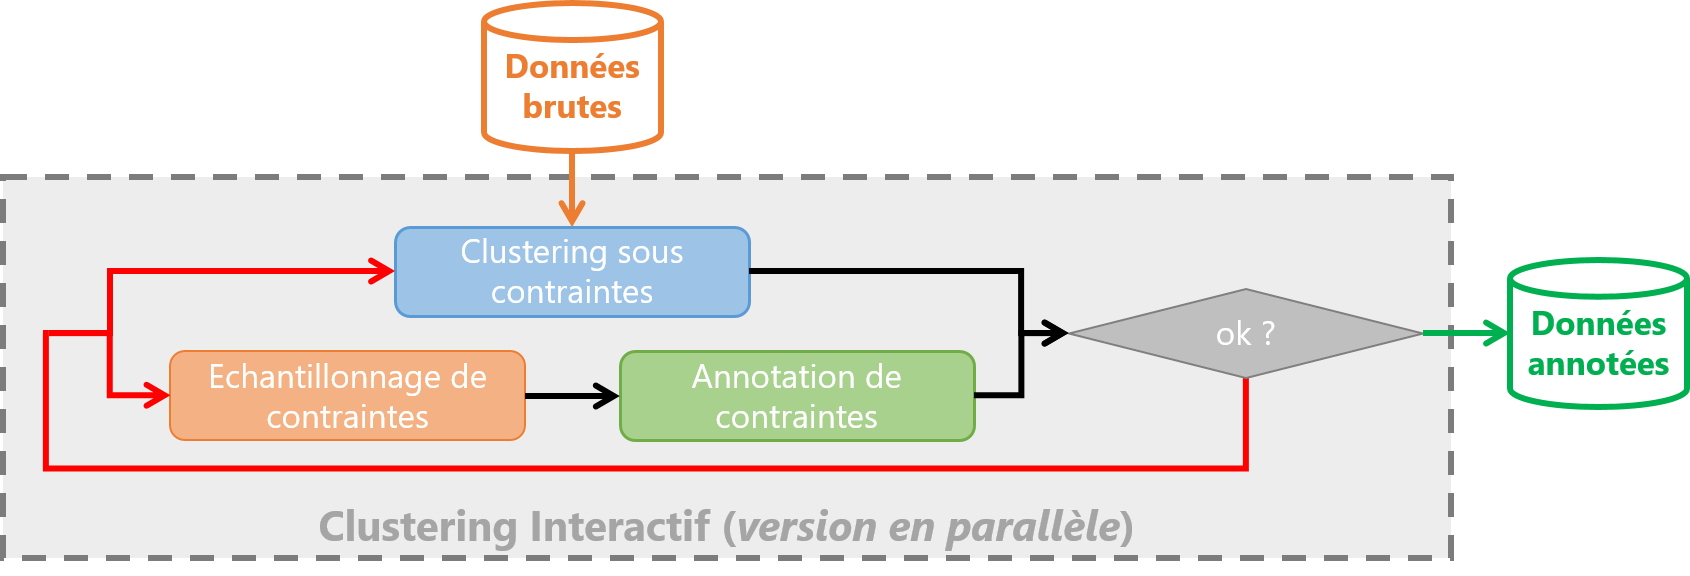
\includegraphics[width=0.95\textwidth]{figures/interactive-clustering-architecture-parallele}
				\caption{
					Schéma illustrant l'architecture du \texttt{Clustering Interactif} en mode parallèle dans le but d'optimiser les temps d'attente entre chaque phase.
					Ainsi, les opérateurs peuvent annoter le temps que la machine propose une nouvelle segmentation des données.
				}
				\label{figure:5.4-GUIDE-PARAMETRAGES-ET-COUTS-ARCHITECTURE-PARALLELE}
			\end{figure}
		\end{leftBarImportantGreen}
		
		\todo[inline]{
			SECTION À RÉDIGER: \\
			- Architecture parallele : pour gagner du temps\\
			- taille de batch d'annotation dépendant de la taille du jeu de données (dépend du temps de clustering)
			- rappeler les équations de temps: environ 24 x taille de dataset, sans les revues d'annotations \\
			- besoin de 3 annotateurs pour confronter les vision et modéliser dans de bonnes conditions. organiser les revues sur la base des différences entre cas d'usage métier \\
			- ajouter de la redondance si le cas d'usage est complexe, mais ça ralenti \\
			- avantage par rapport aux méthode usuelles : moins abstrait/complexe, moins d'essai-erreur
		}